\documentclass[a4paper,oneside,12pt]{book}
%----------------------------------------------------------------------------------------
%	WELCOME!
%   It's probably worth having a read through this file to set up the broad parameters.
%----------------------------------------------------------------------------------------

%----------------------------------------------------------------------------------------
%	COVER PAGE
%   The cover page is laid out in title/title.tex. You can choose a colour
%   or black and white logo
%----------------------------------------------------------------------------------------

%----------------------------------------------------------------------------------------
%	THESIS INFORMATION
%   Put title, author name, degree, type of work, school, department in here
%   It will be used for the title page and for the embedded PDF information
%----------------------------------------------------------------------------------------

\newcommand{\thesistitle}{Learning for sensor-based, real-time fall detection for cyclists.  } % Your thesis title, this is used in the title and abstract
\newcommand{\degree}{B. A (Mod.) Computer Science} % Your degree name, this is used in the title page and abstract
\newcommand{\typeofthesis}{Final Year Project} % dissertation, Final Year Project, report, etc.
\newcommand{\authorname}{Aidan Mongan} % Your name, this is used in the title page and PDF stuff
%% Comment out the next line if you don't want your ID to appear
\newcommand{\authorid}{14334583} % Your ID
\newcommand{\keywords}{this, that, more} % Keywords for your thesis
\newcommand{\school}{\href{http://www.scss.tcd.ie}{School of Computer Science and Statistics}} % Your school's name and URL, this is used in the title page

%% Comment out the next line if you don't want a department to appear
%\newcommand{\department}{\href{http://researchgroup.university.com}{Department Name}} % Your research group's name and URL, this is used in the title page

\AtBeginDocument{
\hypersetup{pdftitle=\thesistitle} % Set the PDF's title to your title
\hypersetup{pdfauthor=\authorname} % Set the PDF's author to your name
\hypersetup{pdfkeywords=\keywords} % Set the PDF's keywords to your keywords
\hypersetup{pdfsubject=\degree} % Set the PDF's keywords to your keywords
}

%% Language and font encodings
\usepackage[T1]{fontenc} 
\usepackage[utf8]{inputenc}
\usepackage[english]{babel}

%% Bibliographical stuff
\usepackage[round,sort,comma,numbers]{natbib}

%% Document size
% include showframe as an option if you want to see the boxes
\usepackage[a4paper,top=2.54cm,bottom=2.54cm,left=2.54cm,right=2.54cm,headheight=16pt]{geometry}

%% Useful packages
\usepackage{amsmath}
\usepackage[autostyle=true]{csquotes} % Required to generate language-dependent quotes in the bibliography
\usepackage[pdftex]{graphicx}
\usepackage[colorinlistoftodos]{todonotes}
\usepackage[colorlinks=true, allcolors=black]{hyperref}
\usepackage{caption} % if no caption, no colon
\usepackage{sfmath} %use sans-serif in the maths sections too
\usepackage[parfill]{parskip}    % Begin paragraphs with an empty line rather than an indent
\usepackage{setspace} % to permit one-and-a-half or double spacing
\usepackage{enumerate} % fancy enumerations like (i) (ii) or (a) (b) and suchlike
\usepackage{booktabs} % To thicken table lines
\usepackage{fancyhdr}

\pagestyle{plain} % Embrace simplicity!

%% The Mechanical engineers require your name and ID on the top of every page.
%% Uncomment the following block if you want your name and ID at the top of
%% (almost) every page.

%\pagestyle{fancy}
%\fancyhf{} % sets both header and footer to nothing
%\renewcommand{\headrulewidth}{0pt}
%\cfoot{\thepage}
%\ifdefined\authorid
%\chead{\it \authorname\ (\authorid)}
%\else
%\chead{\it \authorname}
%\fi
%% End of block

%% It is not a requirement of the university that the font should be sans-serif, but
%% the Mechanical engineers require it. Comment out the following line to disable it
\renewcommand{\familydefault}{\sfdefault} %use the sans-serif font as default

%% If you're not using sans-serif, consider using Palatino instead of the LaTeX standard
%\usepackage{mathpazo} % Use the Palatino font by default if you prefer it to Computer Modern

\renewcommand{\theequation}{\arabic{equation}} %% use continuous equation numbers

%% Format Chapter headings appropriately
\usepackage{titlesec}
\titleformat{\chapter}[hang] 
{\normalfont\huge\bfseries}{\thechapter}{1cm}{} 

\title{\thesistitle}
\author{\authorname}

\frontmatter
\begin{document}
\begin{titlepage}

\center % Center everything on the page

%% All the text parameters should be taken from the start of the main.tex file.
%% You should only alter stuff here if you want to change the layout

%----------------------------------------------------------------------------------------
%	LOGO SECTION
%----------------------------------------------------------------------------------------
%% Choose one of the following -- a colour or black-and-white logo


\includegraphics{title/Trinity_RGB_transparent_main.png}\\[1cm] 
%
\includegraphics[width=12cm]{title/black-stacked-trinity.jpg}\\[1cm] 

\Large \school\\[1.5cm] % Minor heading such as course title
\ifdefined\department
\large \department\\[1.5cm] % Minor heading such as course title
\fi

%----------------------------------------------------------------------------------------
%	TITLE SECTION
%----------------------------------------------------------------------------------------
\makeatletter
{ \huge \bfseries \thesistitle}\\[1.5cm] % Title of your document
 

%----------------------------------------------------------------------------------------
%	AUTHOR SECTION
%----------------------------------------------------------------------------------------

\ifdefined\authorid
\authorname\\ % Your name
\authorid\\[2cm] % Your Student ID
\else
\authorname\\[2cm] % Your name
\fi

%----------------------------------------------------------------------------------------
%	DATE SECTION
%----------------------------------------------------------------------------------------

{\large \today}\\[2cm] % Date, change the \today to a set date if you want to be precise

 
%----------------------------------------------------------------------------------------
%	TYPE OF THESIS SECTION
%----------------------------------------------------------------------------------------
 A \typeofthesis\ submitted in partial fulfilment\\of the requirements for the degree of\\
\degree

\vfill % Fill the rest of the page with whitespace

\end{titlepage}
\pagenumbering{roman}
\section*{\Huge{Declaration}}
\vspace{1cm}
I hereby declare that this project is entirely my own work and that it has not been submitted as an exercise for a degree at this or any other university.

\vspace{1cm}
I have read and I understand the plagiarism provisions in the General Regulations of the University Calendar for the current year, found at \url{http://www.tcd.ie/calendar}.
\vspace{1cm}

I have also completed the Online Tutorial on avoiding plagiarism `Ready Steady Write', located at
\url{http://tcd-ie.libguides.com/plagiarism/ready-steady-write}.
\vspace{3cm}

Signed:~\rule{5cm}{0.3pt}\hfill Date:~\rule{5cm}{0.3pt}

\chapter*{Abstract}
Like all extreme sports, mountain biking comes with the potential for serious injury to the rider in the event of an accident. Non fatal injuries can easily become fatal, when one is alone, far from help and potentially incapacitated. A study conducted by Paracelsus Medical University recorded injury rates as high as 16.8 injuries per 1000 hours of riding, with 22 being moderate and 16 being severe, with rider error being the leading cause \cite{studyOfMTBInjuries}. An automated crash detection system has the potential to be life saving in the worst of circumstances.

Existing discipline-specific solutions e.g., for road only or for mountain use only, on both hardware (Specialized’s AnGi) and software (Strava Beacon,Garmin) have inflexible detection algorithms focusing on using thresholds for only one to two data points. For example AnGi records values from its inbuilt gyroscope and accelerometer, while Garmin’s system uses only accelerometer values. Such threshold-based solutions pose issues in terms of high false detection rates and a single threshold value is unlikely to be suitable for different users at different skill levels.
  
 This project expands on previous research done in the area of wearable fall detection devices for the elderly, focusing on the design of a software solution for real-time fall detection. Three data points are used: raw sensor data from both a tri-axial gyroscope and a tri-axial accelerometer as well as the rate of change of speed, calculated via GPS. The proposed system utilizes learning techniques to improve detection rates and over time generates a more personalized model. Based on pre-captured training data of both regular riding and crashes, data is classified using a multivariable logistic regression model in real-time to determine whether a crash has occurred. Raw sensor data is captured from the inbuilt sensors present on android smartphones.

This approach is implemented as an android application called “RideSafe” and was evaluated using a user study, comprising of X participants at local trail centres over a Y day period. Crash data was also collected, by means of intentional crashes in a controlled environment  for verification.  Results show that this system can successfully detect upwards of X crashes with a low rate of Y false positives….


\newpage
\onehalfspacing\raggedright %\raggedright turns off justification and hypenation

\section*{\Huge{Acknowledgements}}
Thanks Mum!

You should acknowledge any help that you have received (for example from technical staff), or input provided by, for example, a company.
\tableofcontents
%%\listoffigures
%%\listoftables
\newpage


\mainmatter
\chapter{Introduction}

\section{Motivation }

Personal experiences were the main driving factor in my motivation to pursue this study. As a mountain biker with 10 years of experience I have sustained my fair share of minor injuries, but witnessing injuries sustained by more venerable fellow riders are sometimes more impactful. Last summer on a seemingly normal spin with a friend, we discovered a woman lying injured off on the trail side, incapacitated and unable to call for help so I did on her behalf. Multiple phone calls later to aid the first responders in locating us they arrived - around 1 hour after impact.  This experience made me realize how useless your mobile phone is to you in these situations when one is unable to even pick it up.

Currently there are 29,000 registered members of cycling Ireland and with mountain biking  becoming ever more popular each year this number is set to grow. 


\section{Aims}


The  aim of this project was to develop an android application for real-time fall detection for cyclists,  automating the process of requesting assistance, and to reduce response time in the event of an accident. Before development of the application I set myself strict aims to achieve. 

\subsection*{Simplistic and Intuiative}
After the initial set up process, to carry out the main use case: crash detection would be started and stopped with a single press of a button. Start the service, put your phone in your pocket and enjoy your time on you bike with piece of mind. Simple and convenient to use, removing the possibility of confusion for the end user, as the end users will be members of  the general public.
A simple user interface is important as the setting to which the app would be outdoors in potentially harsh weather conditions, external factors such as glare from the sun  and the possibility of moisture on the screen make high detailed, small user interface elements unsuitable. Less is more in this scenario.

\subsection*{Diverse}
Many existing systems are discipline specific, only working for one aspect of cycling i.e., for cross country usage only. I intend this app to have the potential to work for all disciplines of cycling. Targeting single disciplines would drastically reduce the number of potential users as well as producing highly undesirable, inaccurate results if used for the incorrect discipline.

\subsection*{Standalone}
Utilizing android smartphones built in sensors removes the need for extraneous external equipment for ride monitoring.  I intend the app to work as expected with one's phone placed in their pocket or bag, requiring no extra mounting equipment for either the rider or the bike.

\subsection*{Enjoyable user experience}
Many existing solutions exhibit deal breaking issues which ultimately causes the end user to stop using the system, I aim to eradicate the pitfalls present in other systems leading to a better user experience. 

\subsection*{Efficiency}
Performance in terms of battery usage is of utmost importance, heavy battery usage would have the potential to kill the phone when one would need it most - in an emergency. Every possible optimization in terms of battery will be made where possible - without impacting performance.

\section{Personal Goals}
In addition to the aims of this project I had set some personal goals to achieve from undertaking this project.

\subsection*{Devolop a fully functional application.}
Having had brief experience working with android studio before undertaking this project to develop simple applications, most of which were interfaces for arduino circuits connected via bluetooth, I had never developed such a large scale complex application prior to this project. I was excited to broaden my skill set and develop an application ready to be published to the google play store. 

\subsection*{Work with Embedded sensors.}
Having experience working with microcontrollers and various sensors, I was excited to utilize the plethora of available sensors present in android smartphones today. 

\subsection*{Collect and Analyse Real World Data.}
Datasets for what a bike accident looks like in terms of sensor values are few and far between, I was excited to conduct my own research with many unknowns to which I would need to discover. Having very few similar documented studies available I was very interested to study this particular system in the domain of cycling.  

\subsection*{Real world testing.}
I was aware before undertaking this study that it would involve a lot of real world data collection, analysis and testing. Being a crash detection application testing could not be simulated sitting at a desk, which meant all my testing would need to be done in the real world which proved both challenging and exciting.


\section{Readers Guide}
\subsection* {2 - Background}
This section will discuss the concept of fall/accident detection, exploring both the sport and medical applications. The two main approaches of fall detection will be discussed and the strong points as well as issues with each type of system will be discussed.

\subsection* {3 - Design}

here about design 

\subsection* {4 - Implementation}
here about implementation

\subsection* {5 - Evaluation}

evaluation goes here 

\subsection* {6 - Conclusion}

da CONCLUSION



\chapter{Background}
here is the background

\section{The Concept}

what fall detection is all about 

\section{Exsisting Solutions - Medical}

much work has been done .....

\subsection{Vision Based Approaches}
expensive 
privacy issues

\subsection{Sensor Based Approaches}

\section{Exsisting Solutions - Cycling}

\subsection{Garmin}

\subsection{Specilized's ANGI}

\section{Threshold based solutions}

\section {Supervised Machine Learning}

%%\chapter{\LaTeX}
\label{latexchapter}
seeing \LaTeX{}, or more properly ``\LaTeXe{}'', is a very useful document processing program. It is very widely used, widely available, stable and free. Famously, \TeX, upon which \LaTeX{} is built, was originally developed by the eminent American mathematician Donald Knuth because he was tired of ugly mathematics books\cite{shustek2008interview}. Although it has a learning curve (made much less forbidding by online tools and resources -- see below), it allows the writer to concentrate more fully on the content, and takes care of most everything else.

While it can be used as a word processor, it is a \emph{typesetting} system, and Knuth's idea was that it could be used to produce beautiful looking books:
\begin{quote}
\emph{\LaTeX{} is a macro package which enables authors to typeset and print their work at the highest typographical quality, using a predefined, professional layout.}\footnote{This is from \citet{oetiker2001not}. Did we mention that you should minimise your use of footnotes?}
\end{quote}
\LaTeX{} has great facilities for setting out equations and a powerful and very widely supported bibliographic system called BibTeX, which takes the pain out of referencing.

Three useful online resources make \LaTeX~much better:
\begin{enumerate}[(1)]
\item An excellent online \LaTeX{} environment called ``Overleaf'' is available at \url{http://www.overleaf.com} that runs in a modern web browser. It's got this template available -- search for a TCD template. Overleaf can work in conjunction with Dropbox, Google Drive and, in beta, GitHub.
\item Google Scholar, at \url{http://scholar.google.com}, provides BibTeX entries for most of the academic references it finds.
\item An indispensable and very fine introduction to using \LaTeX{} called \emph{``The not so short introduction to LATEX 2$\varepsilon$''} by \citet{oetiker2001not} is online at \url{https://doi.org/10.3929/ethz-a-004398225}. Browse it before you use \LaTeX~for the first time and  read it carefully when you get down to business.
\end{enumerate}
Other tools worth mentioning include:
\begin{itemize}
\item \texttt{Draw.io} -- an online drawing package that can output PDFs to Google Drive -- see \url{https://www.draw.io}.
\end{itemize}
\chapter{Evaluation}
\chapter{Conclusion}

\section {Future Work}

\subsection {Training}

The author believes that the accuracy of RideSafes detection algorithm could greatly be improved with more comprehensive training data. Due to time constraints the data used for training the machine learning model is not as diverse as intended. The training data used for ride safe during tested was collected only from two riders. As discussed throughout even with the most common types of crashes displaying similar patterns, no two riders are identical.   With RideSafe performing as it does one can only deduce performance would improve with a more generalized model to begin with eventually leading to a more personalized model over time.





\subsection {Collaboration}

Currently on the market popular ride tracking applications severely lack  any safeguards for the users safety, popular cycling oriented fitness tracking applications such as Trailforks or Strava actively monitor the users speed and location. Without major redesigns for either party the crash detection logic present in RideSafe could be implemented as a supplementary feature for the benefit of the users. Since the most power intensive feature of RideSafe is GPS functionality, the algorithm could be added to Strava or Trailforks adding only marginally higher power consumption then they already have.




\subsection {Inter-Device communication}
RideSafe would greatly benefit with a companion server. Three major improvements could be made with server-device communication 


\subsection *{Communal Accident HeatMap}

Crash locations collected from all users around the world could be collected to populate a global heatmap accessible to all users. All accident sites from all users could produce an accurate depiction of where danger may be present, potentially saving users from riding dangerous trails or locations. The map could easily be split into an all time accident heatmap as well as showing only recent accidents which could indicate a trail which recently became hazardous, such as a fallen tree or a dislodged rock.



\subsection *{Push Notifications}
Once a crash is detected fellow local users of RideSafe could be sent a distress notification. By locating the nearest users, a distress call could be put out. As the emergency services can take quite a while to arrive, perhaps a local first aider cold reach the scene in advance.




\subsection *{Shared Training Data}
Crash data collected from all users automatically pushed to a server could be used to create a shared dataset of training data, benefiting all users and improving RideSafes generalized model.



\subsection *{Performance Improvements}


As suggested to the author external speedometers for bicycles are readily available and inexpensive. As GPS is currently used to calculate speed in Ridesafe improvements in terms of battery performance and accuracy can be made by using an external speedometer. These Bluetooth enabled devices communicating using ANT+ can be fitted to any bicycle to calculate speed and if utilized device battery life would greatly improve. 

\newpage
\section {Conclusion}

 The purpose of this project was to develop a simple to use crash detection application using machine learning in real-time, and by doing so potentially save someone's life. As shown from the results, this goal was achieved. The author is delighted to have been able to achieve all aims originally set in the planning stage of RideSafe, as well as achieving all the personal goals set in chapter 1. RideSafe may not be ready for a full release at time of writing but the author was adamant to make their presence on the google play store, as shown in figure \ref{store} RideSafe is currently available for open beta testing. Working in an area where specific relevant sensor data is not publically available has been a challenging experience, discovering unknowns, alone has been a very rewarding experience to which the author is extremely proud to have achieved. To the best of the authors knowledge RideSafe is the first sensor based application to use speed as a factor in determining whether a crash has occurred as well as classifying live sensor readings in real-time on a single device.

All functional requirements have been accomplished as well as laying down the foundations for many non-functional requirements. With time constraints as well as the logistics involved with real world testing and training, development of RideSafe has not been an easy feat to complete, however it has been a truly rewarding experience. Choosing to undertake my own idea for a project was daunting at first, with so many unknown variables at play at the beginning I had my doubts at the feasibility of completing this project. My motivation to create an application which one day may save a life kept me focused to reach my end goal. 

 By researching the innovations made in the medical domain as well analysing the pitfalls of existing solutions, the development of RideSafe has shown that existing solutions may not always be the optimal solution. 


%%%%%%%%%%%%%%%%%%%%%%%%%%%%%%%%%%%%%%%%
\begin{figure}[h]
      \centering
      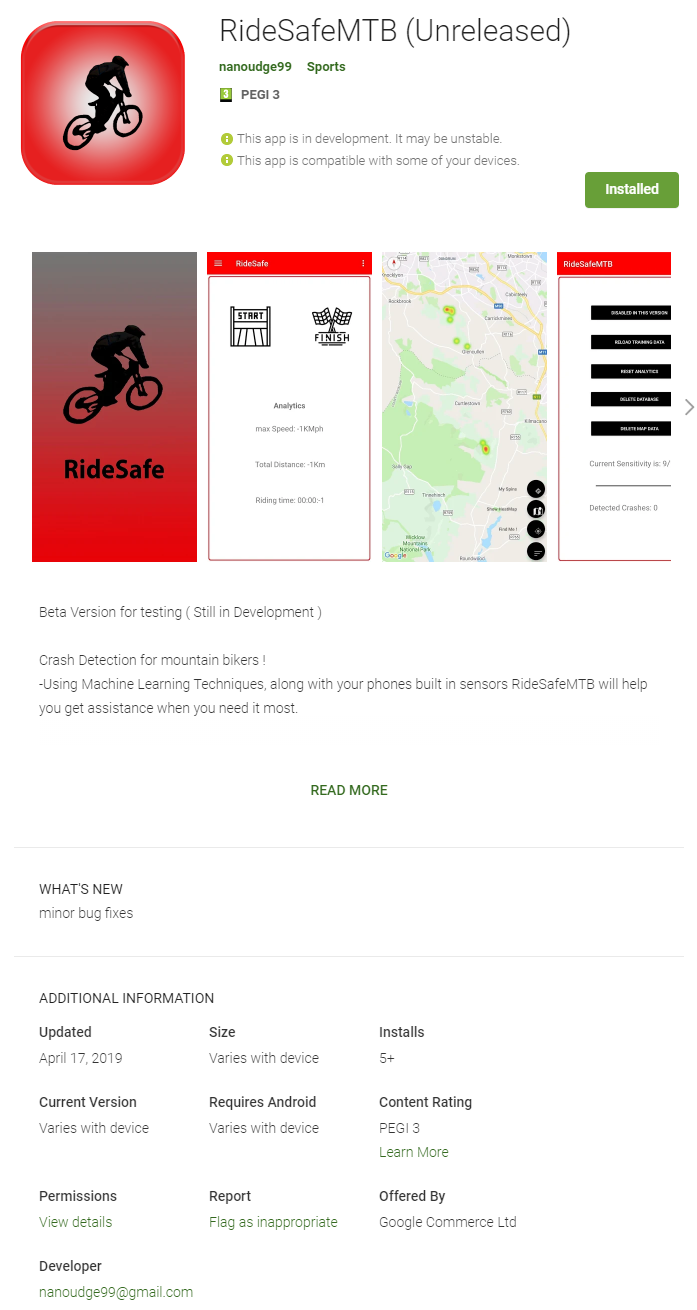
\includegraphics[scale = 1.3]{conclusion/Capture.png}
      \caption{Play Store Listing For RideSafe}
      \label{store}
\end{figure}
%%%%%%%%%%%%%%%%%%%%%%%%%%%%%%%%%%%%%%%%

\bibliographystyle{unsrtnat}
\bibliography{bibs/references}
\appendix
\renewcommand{\thechapter}{A\arabic{chapter}}
\chapter{Appendix}

\section{Other Resources}

A beta version of Ridesafe is currently availible on the Google Play store which can be accessed by folloing this link: https://play.google.com/store/apps/details?id=com.release.nanou.ridesafe

The source code for RideSafe is availible on the authors Github account : https://github.com/monganai/RideSafe


\section{Supplied With This Report}

Supplied with this report is a rescorce containing:

\begin{itemize}
\item The source code for RideSafe as well as a pre-compiled version of the application (.APK File)

\item A subset of collected sensor values used for analyzing and training RideSafe

\end {itemize}

\newpage

\section{Application Screenshots}


%%%%%%%%%%%%%%%%%%%%%%%%%%%%%%%%%%%%%%%%
\begin{figure}[h]
      \centering
      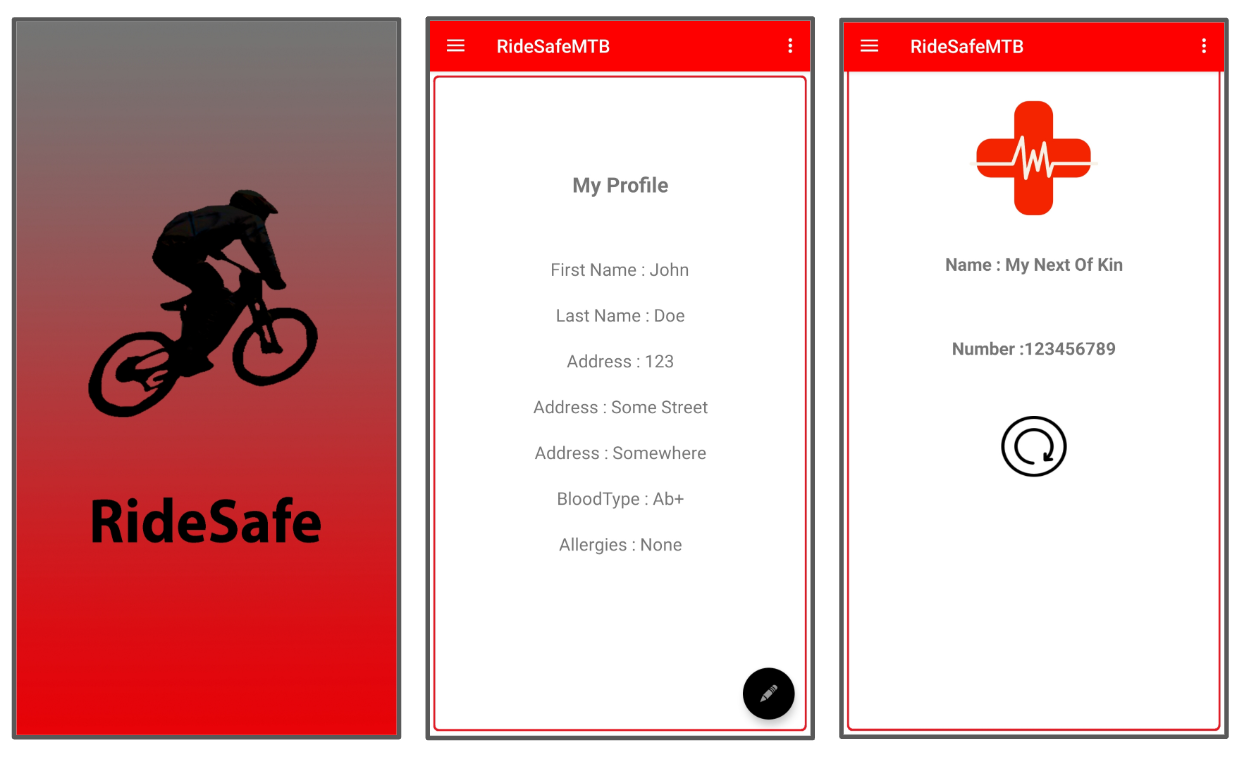
\includegraphics[scale = .9]{appendix/1.png}
      \caption{}
      \label{1}
\end{figure}
%%%%%%%%%%%%%%%%%%%%%%%%%%%%%%%%%%%%%%%%




%%%%%%%%%%%%%%%%%%%%%%%%%%%%%%%%%%%%%%%%
\begin{figure}[h]
      \centering
      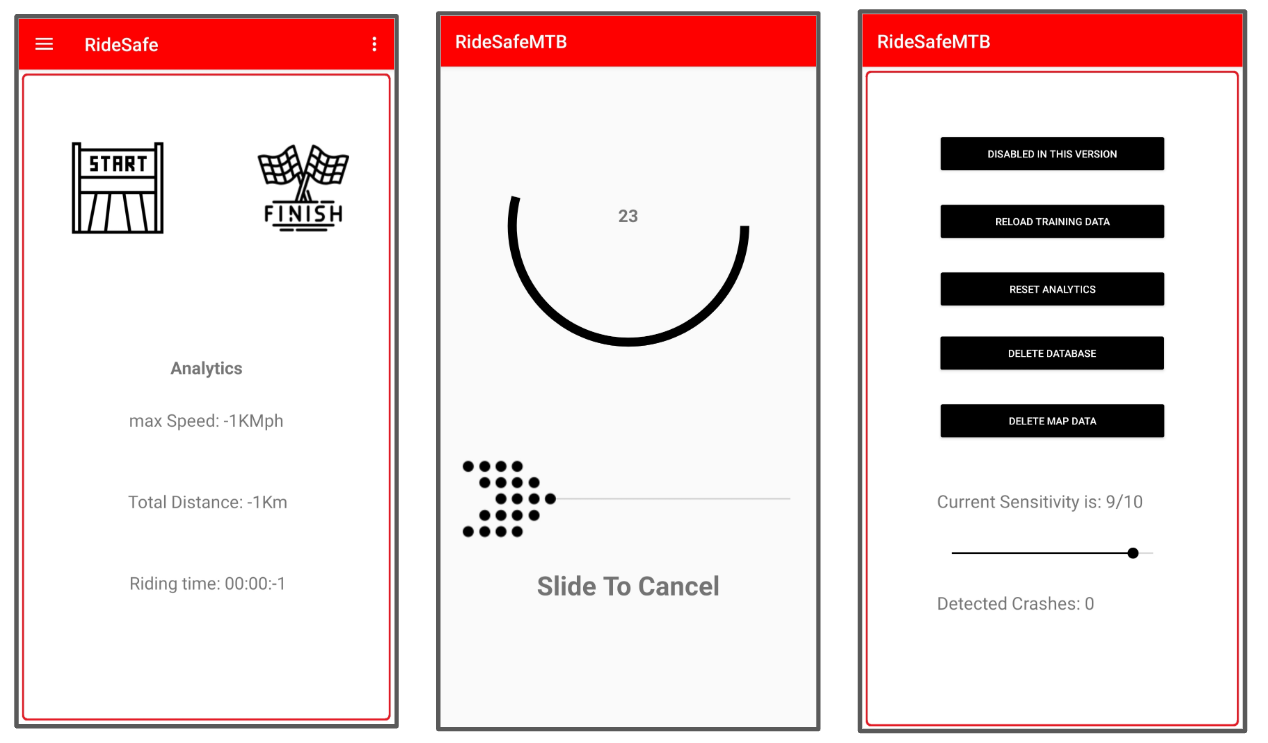
\includegraphics[scale = .9]{appendix/2.png}
      \caption{}
      \label{2}
\end{figure}
%%%%%%%%%%%%%%%%%%%%%%%%%%%%%%%%%%%%%%%%




%%%%%%%%%%%%%%%%%%%%%%%%%%%%%%%%%%%%%%%%
\begin{figure}[h]
      \centering
      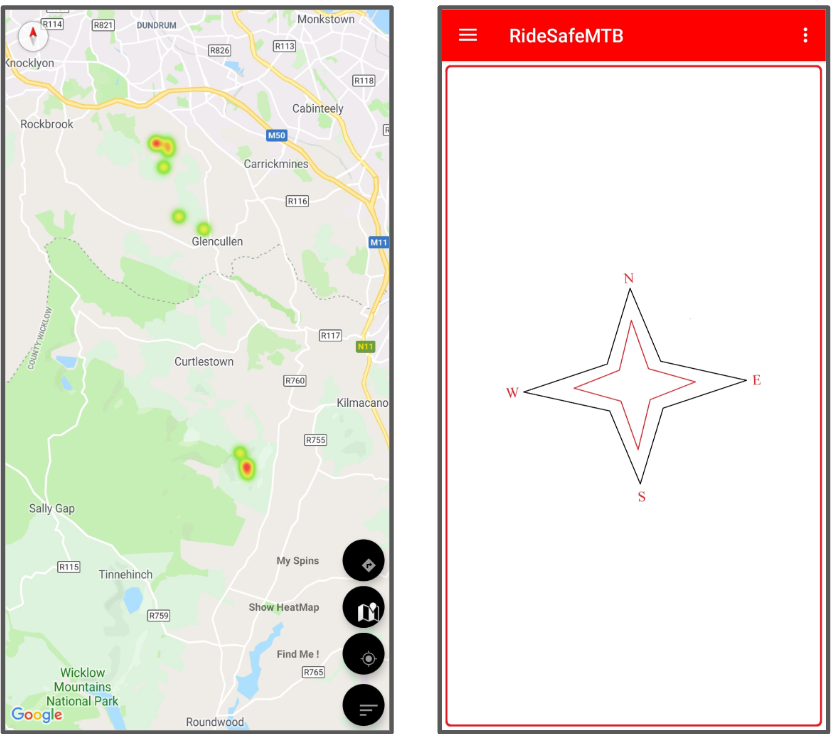
\includegraphics[scale = .9]{appendix/3.png}
      \caption{}
      \label{cm}
\end{figure}
%%%%%%%%%%%%%%%%%%%%%%%%%%%%%%%%%%%%%%%%



\end{document}